  Dieses Kapitel behandelt die Evaluation der Java Web Frameworks. Es wird die
  kombinierte Methode aus dem Kapitel 
  \ref{chapter:MethodenZurEntscheidungsfindungBeiEinerEvaluation}
  (\nameref{chapter:MethodenZurEntscheidungsfindungBeiEinerEvaluation}, S.
  \pageref{chapter:MethodenZurEntscheidungsfindungBeiEinerEvaluation}ff)
  angewendet. Mit der definition von sinnvollen Rahmenbedingungen soll die
  Evaluation durchgeführt und das Resultate in Form einer Rangliste vorgelegt
  werden.
    
  \section{Rahmenbedingungen für die Evaluierung}
  
  Die Rahmenbedingungen für die Evaluierung werden über Soll-Kriterien und
  KO-Kriterien festgelegt.

  \subsection{Soll-Kriterien}
  
  Die Eignung, der zu evaluierenden Java Web Frameworks, wird durch eine Menge
  von Soll-Kriterien bestimmt. Die Soll-Kriterien bestimmen die Anforderungen,
  welche erfüllt werden sollen. Die Anforderungen stammen von einer
  Projektgruppe der Hochschule für Technik und Wirtschaft Berlin. Die
  Soll-Kriterien werden für den Einsatz in der \ac{ZKB} priorisiert.
  
  Soll-Kriterien sind Vorgaben, die möglichst weitgehend Erfüllt werden sollen.
  Wenn ein solches Kriterium nicht erfüllt werden kann, schliesst das die
  Alternative nicht aus. Jedem Soll-Kriterium wird für die Identifikation eine
  eindeutige ID vergeben. Die ID setzt sich folgendermassen zusammen: 
  \{Soll\}-\{Laufnummer\}.
  
  \subsubsection{Anforderungen an Web Frameworks nach AgileLearn}
  
  Eine Projektgruppe namens AgileLearn von der Hochschule für Technik und
  Wirtschaft Berlin befasst sich mit dem Thema Web Frameworks. Die
  Projektgruppe hat sich die Frage gestellt: ``\begin{itshape}Welche
  Anforderungen müssen bei der Wahl eines Webframeworks berücksichtigt
  werden?\end{itshape}''\footnote{Zitat von Raoul Jaeckel, siehe
  \cite{AnforderungenAnWebframeworks}}. Aus der Fragestellung heraus, haben sie
  18 Anforderungen an ein Web Framework ausgearbeitet, welche öffentlich in
  einem Google-Doc\footnote{Ein Service von Google um Dokumente öffentlich zu
  bearbeiten.} ersichtlich sind.
  
  Folgende Anforderungen stammen aus dem Dokument ``\begin{itshape}18
  Anforderungen an Webframeworks -
  OpenDoc\end{itshape}'', siehe \cite{AnforderungenAnWebframeworks}, und werden
  im Anhang \ref{chapter:18AnforderungenNachAgileLearn}
  (\nameref{chapter:18AnforderungenNachAgileLearn}, S.
  \pageref{chapter:18AnforderungenNachAgileLearn}ff) zusammengefasst und mit
  einer ID versehen.

  \subsection{KO-Kriterien}
  
  Anhand einer Menge von KO-Kriterien wird die Auswahl der Alternativen
  eingeschränkt. Die KO-Kriterien sind aus dem \begin{itshape}Handbuch der
  IT-Architektur\end{itshape}, siehe \cite{ZkbHandbuchDerItArchitektur}, der
  \ac{ZKB} entnommen. Die Namensgebung in dem Handbuch unterscheidet sich
  leicht, es wird nicht von KO-Kriterien, sondern von Grundsätzen gesprochen.
  
  KO-Kriterien sind Vorgaben, welche zwingend erfüllt sein müssen. Falls ein
  Kriterium nicht erfüllt werden kann, fällt die Entscheidung auf diese
  Alternative negativ aus. Jedem KO-Kriterium wird für die Identifikation eine
  eindeutige ID vergeben. Die ID setzt sich folgendermassen zusammen: 
  \{KO\}-\{Laufnummer\}.

  \subsubsection{Grundsätze aus der IT-Architektur der Zürcher Kantonalbank}
  
  Ein Grundsatz wird im Handbuch wer IT-Architektur wie folgt definiert:\\
  
  ``\begin{itshape}Es sind Grundsätze definiert, nach denen sich die Baupläne
  der IT-Systeme zu richten haben. Die Grundsätze sind ein Regelwerk mit
  Weisungscharakter.\end{itshape}''
  \footnote{\cite{ZkbHandbuchDerItArchitektur} Kapitel 1.3 - \begin{itshape}Was
  ist die IT-Architektur der ZKB\end{itshape}, Seite 11}
  \\
  \\
  \noindent
  Dabei gibt es eine Hintertür:\\

  ``\begin{itshape}Grundsätze sind verbindliche Vorgaben (Konventionen), von
  denen nur in begründeten Ausnahmen abgewichen werden kann.\end{itshape}''
  \footnote{\cite{ZkbHandbuchDerItArchitektur} Kapitel 1.8 -
  \begin{itshape}Leseanleitung\end{itshape}, Seite 14}
  \\
  \\
  \noindent
  Das Dokument wurde analysiert und alle Grundsätze, welche für diese
  Diplomarbeit relevanten sind, werden im Anhang
  \ref{chapter:GrundsaetzeDerZkbItArchitektur}
  (\nameref{chapter:GrundsaetzeDerZkbItArchitektur}, S.
  \pageref{chapter:GrundsaetzeDerZkbItArchitektur}ff) aufgelistet und mit einer
  ID versehen.

  \section{Priorisierung der Soll-Kriterien}
  
  Da 18 Soll-Kriterien definiert wurden und diese in jeder Alternative 
  untersucht werden müssten, würde das den Rahmen der Diplomarbeit sprengen.
  Desshalb sollen die Soll-Kriterien in eine Hirarchie entsprechend ihrer
  Wichtigkeit für die \ac{ZKB} aufgeteilt werden. Die Hirarchie wird in drei
  Gruppen aufgeteilt:
  
  \begin{itemize}
    \item Wichtig
    \item Nice to have
    \item Unwichtig
  \end{itemize}
  
  Es sollen nur die ``wichtigen'' Soll-Kriterien in die Evaluation mit
  einbezogen werden.
  
  \subsection{Wichtige Aspekte im Software-Lebenszyklus für die ZKB}
  
  \begin{description}
    \item[Sicherheit]
    Nur eine Bank, die als sicher gilt, hat das Vertrauen der Kunden und somit
    Erfolg in ihrem Geschäft.
    \item[Kosten]
    Die laufenden Kosten sollen so tief wie möglich gehalten werden. Gemäss
    Abbildung \ref{img:softwareLifecycleCost} liegen die Hauptkosten im
    Software-Lebenszyklus bei der Maintenance-Phase. Somit können die Kosten für
    requirements Engineering, Design, Programming und Integration vernachlässigt
    werden.
    \item[Ressourcen]
    Damit Software entwickelt und gewartet werden kann, wird die Verfügbarkeit
    von qualifizierten Ressourcen benötigt.
    \item[Image]
    Um sich von der Konkurenz abzuheben wird ein Image aufgebaut das sich
    zeitgemäss, flexibel und inovativ präsentieren soll, siehe
    \cite{WillkommenBeiDerZkb} S. 34ff.
  \end{description}
  
  \begin{figure}[ht]
    \begin{center}
      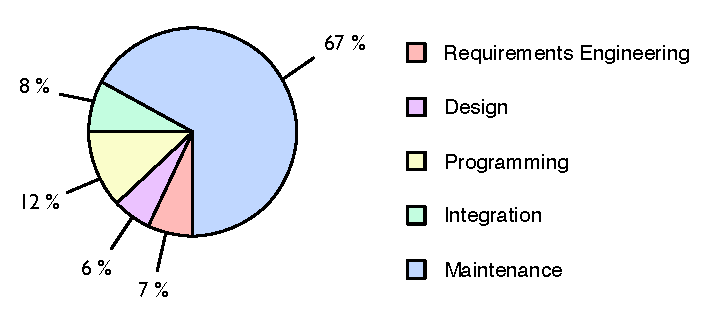
\includegraphics[width=0.7\textwidth]{./image/softwareLifeCycleCost.pdf}
      \caption{Ungefähre relative Kosten der Phasen des Software-Lebenszyklus
      (nach \cite{SoftwareEngineering} S. 11 und
      \cite{SoftwareLifeCycleModels})}
      \label{img:softwareLifecycleCost}
    \end{center}
  \end{figure}
  
  Es soll eine Konsolidierung statt finden, zwischen den 18 Soll-Kriterien und
  den wichtigen Aspekten im Software-Lebenszyklus für die \ac{ZKB}. Die
  Konsolidierung wird in der Tabelle \ref{tab:kosolidierungDerSollKriterien}
  gezeigt.
  
  \begin{table}[!h]
    \sffamily 
    \begin{center}
      \begin{threeparttable}
        \begin{tabular}{p{9cm}cccc}
          \toprule
          Anforderung & (Si) & (Ko) & (Re) & (Im)\\
          \midrule
          \ref{itm:Soll-01} & ++ &    &    &    \\
          \ref{itm:Soll-02} & +  &    &    &    \\
          \ref{itm:Soll-03} &    & ++ &    &    \\
          \ref{itm:Soll-04} &    & +  &    &    \\
          \ref{itm:Soll-05} &    &    &    &    \\
          \ref{itm:Soll-06} & +  & ++ &    & ++ \\
          \ref{itm:Soll-07} &    &    &    &    \\
          \ref{itm:Soll-08} &    &    &    &    \\
          \ref{itm:Soll-09} &    &    &    &    \\
          \ref{itm:Soll-10} &    &    &    &    \\
          \ref{itm:Soll-11} &    &    &    &    \\
          \ref{itm:Soll-12} &    & ++ &    &    \\
          \ref{itm:Soll-13} &    &    & ++ &    \\
          \ref{itm:Soll-14} &    & +  &    &    \\
          \ref{itm:Soll-15} &    &    &    &    \\
          \ref{itm:Soll-16} &    &    &    &    \\
          \ref{itm:Soll-17} &    &    & +  &    \\
          \ref{itm:Soll-18} &    &    &    & ++ \\
          \bottomrule
        \end{tabular}
        \caption{Wie wichtig sind die Soll-Kriterien für die ZKB.}
        \label{tab:kosolidierungDerSollKriterien}
        \medskip 
        %\footnotesize\textbf{Legende:}\smallskip 
        \begin{tablenotes}[++]\footnotesize 
          \item[(Si)] Sicherheit 
          \item[(Ko)] Kosten in der Maintenance Phase des Software-Lebenszyklus
          \item[(Re)] Ressourcen 
          \item[(Im)] Image
          \item[++] hat grossen Einfluss
          \item[+] hat Einfluss
        \end{tablenotes} 
      \end{threeparttable}
    \end{center}
  \end{table}
  
  Die Soll-Kriterien mit zwei oder mehr + werden als ``wichtig'', mit einem
  + als ``nice to have'' und ohne + als ``nicht wichtig'' priorisiert.
  
  \subsection{Wichtig}
  
  \begin{description}
  \item[Soll-01 - Zugriffskontrolle 
  (Authentifizierung/Authorisation/Rollenverwaltung)]
  Auf die Sicherheit von Applikationen in einer Bank wird grossen Wert
  gelegt. Mit einer genügenden Authentifizierung, Authorisation und
  Rollenverwalung, kann eine Applikation sicher implementiert werden.
  
  \item[Soll-03 - Modulare Architektur]
  Um wärend der Maintenance-Phase des Software-Lebenszyklus notwendige
  Anpassungen an einer Applikation machen zu können, ist eine modulare
  Architekur von grossem Vorteil. Zudem ist das auch wärend der
  Entwicklungs-Phase hilfreich.
  
  \item[Soll-06 - Testing]
  Um wärend der Maintenance-Phase des Software-Lebenszyklus notwendige
  Anpassungen an einer Applikation machen zu können, ist ein gutes Testing von
  grossem Vorteil. Das Testing hat auch einen grossen Einfluss auf das Image,
  denn wer möchte schon fehlerhafte Software verwenden. Durch eine gute
  Testbasis, kann auch die Sicherheit einer Applikation gesteigert werden.
  
  \item[Soll-12 - Dokumentation]
  Eine saubere und verständliche Dokumentation eines Web Application Frameworks
  ist das A und O um während allen Software-Lebenszyklen effizient arbeiten zu
  können. Ein Web Application Framework mit einer brillianten Dokumentation hat
  bestimmt höhere Chancen sich längerfristig am Markt durchzusetzten.
  
  \item[Soll-13 - Community]
  Damit die notwendigen Ressourcen, für die Umsetztung und Wartung eines
  Software-Projekts gefunden werden, wird eine entsprechend grosse Community
  benötigt. Wenn die Community genügend gross ist, kann man davon ausgehen,
  dass auch in der Zukunft noch genügend Ressourcen in diesem Bereich
  erreichbar sind.
  
  \item[Soll-18 - AJAX-Unterstützung]
  In der Zeit von Google Mail, Facebook und Twitter wird die Verwendung von
  \ac{Ajax} unterstützten Web Applikationen zur Gewohnheit. Um mit einer Web
  Applikation ein zeitgemässes, flexibles und innovatives Image vermitteln zu
  können, sollten diese mit Ajax-Unterstütztung gebaut werden.
  
  \end{description}
  
  \subsection{Nice to have}
  
  \begin{description}
  \item[Soll-02 - Form-Validierung]
  Eine saubere Form-Validierung gehört zu den notwendigen Werkzeugen, um eine
  sichere Web Applikation zu entwickeln. Dennoch kann durch gutes Testing und
  eine sichere Zugriffskontrolle der selbe Effekt erzielt werden.
  
  \item[Soll-04 - Schnittstellen und Webservices]
  Durch die breite Unterstützung von Schnittstellen und Webservice Technologien
  in der Java Welt, muss ein Web Framework dies nicht schon von Haus aus
  mitbringen. Fall es doch vorhanden ist, um so besser.
  
  \item[Soll-14 - IDE-Unterstuetzung]
  Eine IDE-Unterstützung ist zu präferieren, soll aber kein Hinderniss für den
  Einsatz eines guten Web Frameworks sein.
  
  \item[Soll-17 - Lernkurve fuer EntwicklerInnen]
  Durch die Unterstützung einer soliden Community und einer guten Dokumentation
  kann die Lernkurve beträchtlich beeinflusst werden.
  
  \end{description}
  
  \subsection{Unwichtig}
  
  \begin{description}
  \item[Soll-05 - MVC-Entwurfsmuster]
  Das \ac{MVC} Konzept ist sicher gut, sollte aber nicht eine Anforderung an ein
  Web Framework sein, da es ebenbürdige Alternativen gibt, eine nennenswerte währe
  \ac{MVP}.
  
  \item[Soll-07 - Internationalisierung und Lokalisierung]
  Die \ac{ZKB} hat ihr Geschäftsfeld im Kanton Zürich. Somit ist eine
  Internationalisierung und Lokalisierung nicht wirklich nötig. Da die \ac{ZKB}
  im Auftrag des Kantons handelt, gehe ich davon aus, dass sich das nicht so
  schnell ändern wird.
  
  \item[Soll-08 - Object Relational Mapping (ORM)]
  In der Java Welt git es viele \ac{ORM} Lösungen, welche sich in den Jahren
  durchgesetzt haben, ein paar nennenswerte sind Hibernate, TopLink und
  EclipseLink. Da es Sache des Applikationsservers ist, welches \ac{ORM}
  verwendet wird, stellt dies keine Anforderung an ein Java Web Framework.
  
  \item[Soll-09 - Scaffolding / Rapid Prototyping]
  Mit Scaffolding und Rapid Prototyping kann in der Programmier-Phase des
  Software-Lebenszyklus die Arbeit erleichtert werden. In der Maintenance-Phase
  ergibt sich daraus kein Benefit.
  
  \item[Soll-10 - Caching]
  Caching kann bei Webseiten mit viel statischen Content die Datenmenge, die
  übertragen wird, enorm reduzieren. Bei Business-Applikationen, die über eine
  Rollenverwaltung verfügen, sind die Daten die übertragen werden, meistens sehr
  individuell. Somit besteht keine Nachfrage nach Caching
  
  \item[Soll-11 - View-Engine]
  Da Java eine Objekt Orientierte Sprache ist, wird das schon von der Sprache
  her unterstützt.
  
  \item[Soll-15 - Kosten fuer Entwicklungswerkzeuge]
  Die Kosten der Entwicklungswerkzeuge haben keinen Einfluss auf die
  Maintenance-Phase des Software-Lebenszyklus. Zudem gibt es genügend \acp{IDE}
  für Java, die Open Source sind. Ein Paar nennenswerte sind Eclipse, NetBeans
  und IntelliJ.
  
  \item[Soll-16 - Eignung fuer agile Entwicklung]
  Die Ansätze von Scrum und extreme Programming werden in der \ac{ZKB} je länger
  je mehr angewendet. Dennoch hat das keinen Einfluss auf die Maintenance-Phase
  des Software-Lebenszyklus.
  
  \end{description}
  
  \section{Auswahl der Java Web Frameworks}
  
  Es sollen vier Java Web Frameworks für die Evaluation ausgewählt werden. Ein
  Java Web Framework, das in Frage kommt, wird Alternative genannt. Jede
  Alternative wird mit einer ID in der Form \{A\}-\{Laufnummer\} versehen.
  
  \subsection{Begründung}
  
  Es soll für jede Alternative der Grund der Wahl erläutert werden. In Absprache
  mit dem Projektbetreuer sollen aus den verschiednen Typen von Java Web
  Frameworks jeweils eines gewählt werden. Es wurden folgende Typen definiert:
  
  \begin{itemize}
    \item \ac{RIA} - Frameworks
    \item MVC - Frameworks
    \item Java Script/HTML/CSS - Cross-Compiler Frameworks
    \item In der \ac{ZKB} bereits eingesetzte Frameworks
  \end{itemize}
  
  \subsubsection{A-1 - ULC, Canoo RIA Suite}
  
  ULC, Canoo RIA Suite zählt zu den \ac{RIA} Frameworks. Gemäss Kick-off
  Protokoll Beschluss soll dieses Framework als Alternative gewählt werden.
  Zudem wird die ULC, Canoo RIA Suite in den schweizer Banken Credit Suisse und
  UBS eingesetzt.
  
  \subsubsection{A-2 - Struts 1.3.10 mit ZIP-Framework}
  
  MVC - Framework, das in der ZKB bereits eingesetzt wird.
  
  \subsubsection{A-3 - Vaadin 6.5.7}
  
  Vaadin zählt zu den Java Script/HTML/CSS - Cross-Compiler Frameworks und baut
  auf \ac{GWT} auf.
  
  \subsubsection{A-4 - Apache Wicket 1.4.17}
  
  Ein Framework das in der ZKB bereits eingesetzt wird. An dieser Stelle ist zu
  erwähnen, dass der Einsatz aufgrund von Ausnahmegenehmigungen eingesetzt
  werden darf. Diese müssten im Falle einer erfolgreichen Evaluation ebenfalls
  beantragt werden.

  \section{KO-Kriterien die nicht beachtet werden sollen}
  
  Damit die Durchführung der Evaluation einen Sinn ergibt, sollen einige
  KO-Kriterien nicht beachtet werden. In Absprache mit dem Fachbetreuer der
  \ac{ZKB} betrifft das folgende KO-Kriterien, die im Rahmen der Diplomarbeit
  nicht berücksichtigt werden:
  
  \begin{itemize}
    \item \ref{itm:KO-09} - Für Java-Applikationen (Internet, Extranet und
    Intranet) wird das ZIP-Framework eingesetzt.
    \item \ref{itm:KO-16} - Die Internet-Applikationen funktionieren auch
    eingeschränkt, ohne dass die Skript-Funktion im Browser aktiviert ist.
    \item \ref{itm:KO-20} - Für Ultra Thin Clients bzw. Browser-basierende
    Applikationen muss das aktuelle, Struts-basierende HTML-Client-Framework
    der ZKB Internet Plattform verwendet werden.
  \end{itemize}
  
  \section{Prüfen der zu beachtenden KO-Kriterien}
  
  Es soll eine Prüfung aller Frameworks statt finden, ob es gegen definierte
  KO-Kriterien verstösst. Falls das der Fall ist, wird das Framework von der
  Evaluation ausgeschlossen. In Absprache mit dem Fachbetreuer der \ac{ZKB} gibt
  es gewisse KO-Kriterien, die im Rahmen der Diplomarbeit ausser Kraft treten,
  diese sollen nicht beachtet werden.

  \subsection{A-1 - ULC, Canoo RIA Suite}
  
  Leider wurde wärend der Analyse festgestellt, dass die ULC, Canoo RIA Suite
  nur in einer Java Virtual Machine\footnote{Die Java Virtual Machine ist der
  Teil der \ac{JRE}, der für die Ausführung des Java-Bytecodes verantwortlich
  ist, siehe \cite{JavaVirtualMachine}.} lauffähig ist. Das wird über die
  Technik von Java-Web-Start\footnote{Java-Web-Start ist eine Technik von
  Oracle (damals entwickelt von Sun Microsystems), die es ermöglicht, Java-Anwendungen
  über das Internet mit nur einem Klick zu starten. Im Unterschied zu
  Java-Applets benötigen Java-Web-Start-Anwendungen keinen Browser, um ablaufen
  zu können, siehe \cite{JavaWebStart}.} oder mit der Hilfe von einem
  Java-Applet\footnote{Ein Java-Applet ist ein Computerprogramm, das in der
  Programmiersprache Java verfasst wurde und normalerweise in einem Webbrowser
  ausgeführt wird, siehe \cite{JavaApplet}.} vollbracht. Das ist ersichtlich im
  ULC Architektur Guide, siehe \cite{ULCArchitectureGuide} S. 18. Damit
  verstösst diese Alternative gegen die KO-Kriterien \ref{itm:KO-18} und
  \ref{itm:KO-19}. Aufgrund des Vorgehens aus der Abbildung
  \ref{img:ablaufEvaluation} wird diese Alternative aus der Evaluation
  ausgeschlossen.
  
  Der Client könnte auch als standalone Client implementiert oder in einen
  bestehenden Client integriert werden. Das nützt nichts, da diese Situation
  bereits mit den Java Swing Clients besteht, und abgelöst werden soll.
  
  Falls sich die Grundsätze der IT-Architektur der \ac{ZKB} in der Zunkunft
  dahingehend ändern, dass Java Web Start oder Java Applets verwendet werden
  dürften, stellt die ULC, Canoo RIA Suite ein gute Alternative zur Ablösung
  bestehender Swing Applikationen.
  
  \subsection{A-2 - Struts 1.3.10 mit ZIP-Framework}
  
  Es wurde keine KO-Kriterien gefunden, die für diese Alternative zutreffen.
  
  \subsection{A-3 - Vaadin 6.5.7}
  
  Es wurde keine KO-Kriterien gefunden, die für diese Alternative zutreffen.

  \subsection{A-4 - Apache Wicket 1.4.17}
  
  Es wurde keine KO-Kriterien gefunden, die für diese Alternative zutreffen.
    
  \section{Gewichtete Nutzwertanalyse mit dem Analytic Hirarchy Process}
  
  Es sollen die Soll-Kriterien, auf welche die Frameworks verglichen werden,
  bestimmt werden. Danach soll nach der Methode des \ac{AHP} die Gewichtung der
  Soll-Kriterien vorgenommen und, zur Berechnung der Nutzwertanalyse,
  verwendet werden. Für jede mögliche Alternative soll der Erfüllungsgrad der
  Soll-Kriterien bestimmt und, zur Berechnung der Nutzwertanalyse, vewendet
  werden. Das Resultat der Nutzwertanalyse soll dargestellt werden.
  
  \subsection{Bestimmen der Kriterien}
  
  Die Kriterien, welche in die Evaluation miteinbezogen werden, und somit für
  jede Alternative untersucht werden soll, sind die ``wichtigen''
  Soll-Kriterien:
  
  \begin{itemize}
    \item Soll-01 - Zugriffskontrolle 
    (Authentifizierung/Authorisation/Rollenverwaltung)
    \item Soll-03 - Modulare Architektur
    \item Soll-06 - Testing
    \item Soll-12 - Dokumentation
    \item Soll-13 - Community
    \item Soll-18 - AJAX-Unterstützung
  \end{itemize}
  
  \subsection{Bestimmen der Gewichte mit dem Analytic Hirarchy Process}
  
  Die Bestimmung der Gewichte wird über die Methode des \ac{AHP} gemacht. Für
  den Vergleich der Soll-Kriterien wird die Frage - \begin{itshape}``Wie
  wichtig ist das Soll-Kriterium für die \ac{ZKB}?''\end{itshape} - gestellt.
  
  Es werden alle ``wichtigen'' Soll-Kriterien miteinander verglichen. Die
  Vergleichsmatrix und die daraus resultierende Gewichtung ist in der Tabelle
  \ref{tab:gewichtungDerSollKriterien} und der Abbildung
  \ref{img:gewichtungSollKriterien} ersichtlich. Für die Werte in der
  Vergleichsmatix wird die Skala der Vergleichsgrad, siehe Tabelle
  \ref{tab:vergleichsgrade}, verwendet.
  
  Um die Gewichte anhand der erstellten Vergleichsmatix zu berechnen, wird das
  Java Programm JAHP 2.1 verwendet.
  
  Der Inkonsistenzfaktor beträgt 0.04754 und ist somit sehr klein. Die
  getroffenen Annahmen der Gewichtung sollten desshalb aussagekräftig sein.
  \newline
  
  \begin{table}[!h]
    \sffamily 
    \begin{center}
      \begin{tabular}{l|cccccc|r}
        \toprule
        Vergleich & Soll-01 & Soll-03 & Soll-06 & Soll-12 & Soll-13 & Soll-18
        & Gewichtung\\
        \midrule
        Soll-01 & 1 & 5 & 3 & 5 & 5 & 3 & 34.81 \%\\
        Soll-03 & $\frac{1}{5}$ & 1 & $\frac{1}{3}$ & 1 & 1 & $\frac{1}{5}$ &
        5.91 \%\\
        Soll-06 & $\frac{1}{3}$ & 3 & 1 & 3 & 3 & 1 & 17.93 \%\\
        Soll-12 & $\frac{1}{5}$ & 1 & $\frac{1}{3}$ & 1 & $\frac{1}{3}$ &
        $\frac{1}{5}$ & 4.85 \% \\
        Soll-13 & $\frac{1}{5}$ & 1 & $\frac{1}{3}$ & 3 & 1 & $\frac{1}{5}$ &
        9.07 \%\\ Soll-18 & $\frac{1}{3}$ & 5 & 1 & 5 & 5 & 1 & 27.43 \%\\
        \bottomrule
      \end{tabular}
      \caption{Vergleichsmatrix der Soll-Kriterien nach der Methode des AHP.}
      \label{tab:gewichtungDerSollKriterien}
    \end{center}
  \end{table}
  
  \begin{figure}[ht]
    \begin{center}
      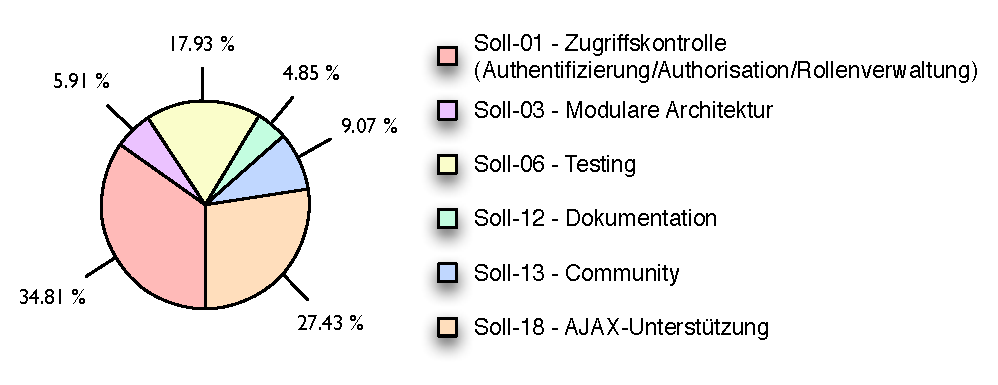
\includegraphics[width=0.95\textwidth]{./image/gewichtungSollKriterien.pdf}
      \caption{Gewichtung der Soll-Kriterien nach der Methode des AHP}
      \label{img:gewichtungSollKriterien}
    \end{center}
  \end{figure}
  
  \subsection{Bestimmen des Erfüllungsgrades}
  
  Für die Werte zur Bestimmung der Erfüllungsgrade wird die Skala der
  Erfüllungsgrade, siehe Tabelle \ref{tab:erfuellungsgrade}, verwendet.
  
  \section{Resultat}
  
  \subsection{A-1 - ULC, Canoo RIA Suite}
  
  Wurde aufgrund der KO-Kriterien \ref{itm:KO-18} und \ref{itm:KO-19} aus der
  Evaluation ausgeschlossen.
  
  \subsection{A-2 - Struts 1.3.10 mit ZIP-Framework}
  
  Siehe Tabelle \ref{tab:nwaA2}.
  
  \begin{table}[ht]
    \sffamily 
    \begin{center}
      \begin{tabular}{l|rrr}
        \toprule
        Kriterien & Gewichtung \(g\) & Erfüllungsgrad \(e\) & Wertigkeit
        \(_A-_2\) \\
        \midrule
        Soll-01   & 34.81 \% & x & y \\
        Soll-03   &  5.91 \% & x & y \\
        Soll-06   & 17.93 \% & x & y \\
        Soll-12   &  4.85 \% & x & y \\
        Soll-13   &  9.07 \% & x & y \\
        Soll-18   & 27.43 \% & x & y \\
        \midrule
        \midrule
        Ergebnis  & 100.00 \% &   & z \\
        \bottomrule
      \end{tabular}
      \caption{Nutzwertanalyse der Alternative A-2 - Struts 1.3.10 mit
      ZIP-Framework}
      \label{tab:nwaA2}
    \end{center}
  \end{table}
  
  \subsection{A-3 - Vaadin 6.5.7}
  
  Siehe Tabelle \ref{tab:nwaA3}.
  
  \begin{table}[ht]
    \sffamily 
    \begin{center}
      \begin{tabular}{l|rrr}
        \toprule
        Kriterien & Gewichtung \(g\) & Erfüllungsgrad \(e\) & Wertigkeit
        \(_A-_3\) \\
        \midrule
        Soll-01   & 34.81 \% & x & y \\
        Soll-03   &  5.91 \% & x & y \\
        Soll-06   & 17.93 \% & x & y \\
        Soll-12   &  4.85 \% & x & y \\
        Soll-13   &  9.07 \% & x & y \\
        Soll-18   & 27.43 \% & x & y \\
        \midrule
        \midrule
        Ergebnis  & 100.00 \% &   & z \\
        \bottomrule
      \end{tabular}
      \caption{Nutzwertanalyse der Alternative A-3 - Vaadin 6.5.7}
      \label{tab:nwaA3}
    \end{center}
  \end{table}
  
  \subsection{A-4 - Apache Wicket 1.4.17}
  
  Siehe Tabelle \ref{tab:nwaA4}.
  
  \begin{table}[ht]
    \sffamily 
    \begin{center}
      \begin{tabular}{l|rrr}
        \toprule
        Kriterien & Gewichtung \(g\) & Erfüllungsgrad \(e\) & Wertigkeit
        \(_A-_4\) \\
        \midrule
        Soll-01   & 34.81 \% & x & y \\
        Soll-03   &  5.91 \% & x & y \\
        Soll-06   & 17.93 \% & x & y \\
        Soll-12   &  4.85 \% & x & y \\
        Soll-13   &  9.07 \% & x & y \\
        Soll-18   & 27.43 \% & x & y \\
        \midrule
        \midrule
        Ergebnis  & 100.00 \% &   & z \\
        \bottomrule
      \end{tabular}
      \caption{Nutzwertanalyse der Alternative A-4 - Apache Wicket 1.4.17}
      \label{tab:nwaA4}
    \end{center}
  \end{table}
